% ============================================================
% Sección 3
% ============================================================
\section{3 EDO Lineal no Homogénea}

\begin{tcolorbox}[enunciado]
\textbf{Clases:}
\begin{itemize}[leftmargin=*]
    \item Video 3) EDO Lineal 1er Orden Homogénea y Variación de Parámetros MCA4 23Sep26
    \item Video 4) Método de Factor Integrante en EDO lineal no Homogénea con Ejemplo MCA4 28Sep26
\end{itemize}
\end{tcolorbox}

\subsection*{ACTIVIDADES}

\begin{enumerate}[label=\arabic*., leftmargin=*]
    \item \textbf{Buffer con llegadas periódicas.} \\
    Replica la información y solución por Variación de Parámetros que se dio a este problema en la clase del 23 de Septiembre (Video 3).
    \subsection*{Solución}
    \begin{figure}[H]
        \centering
        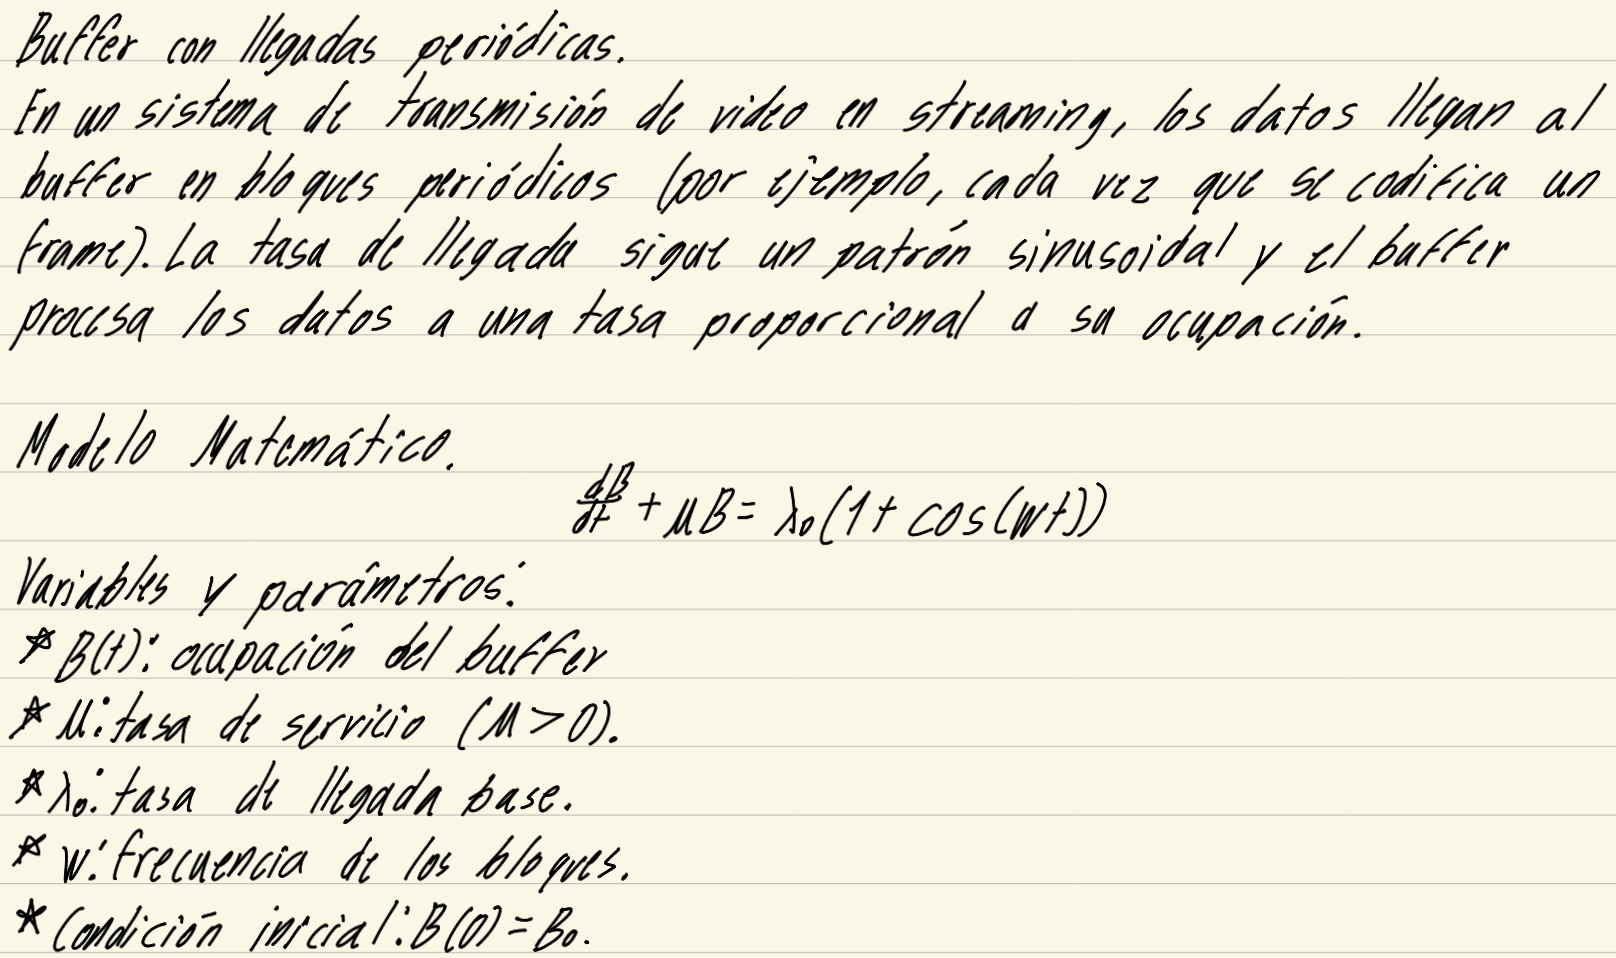
\includegraphics[width=0.8\linewidth]{imagenes/tarea/03_ejercicio/01_image.png}
    \end{figure}

    \begin{figure}[H]
        \centering
        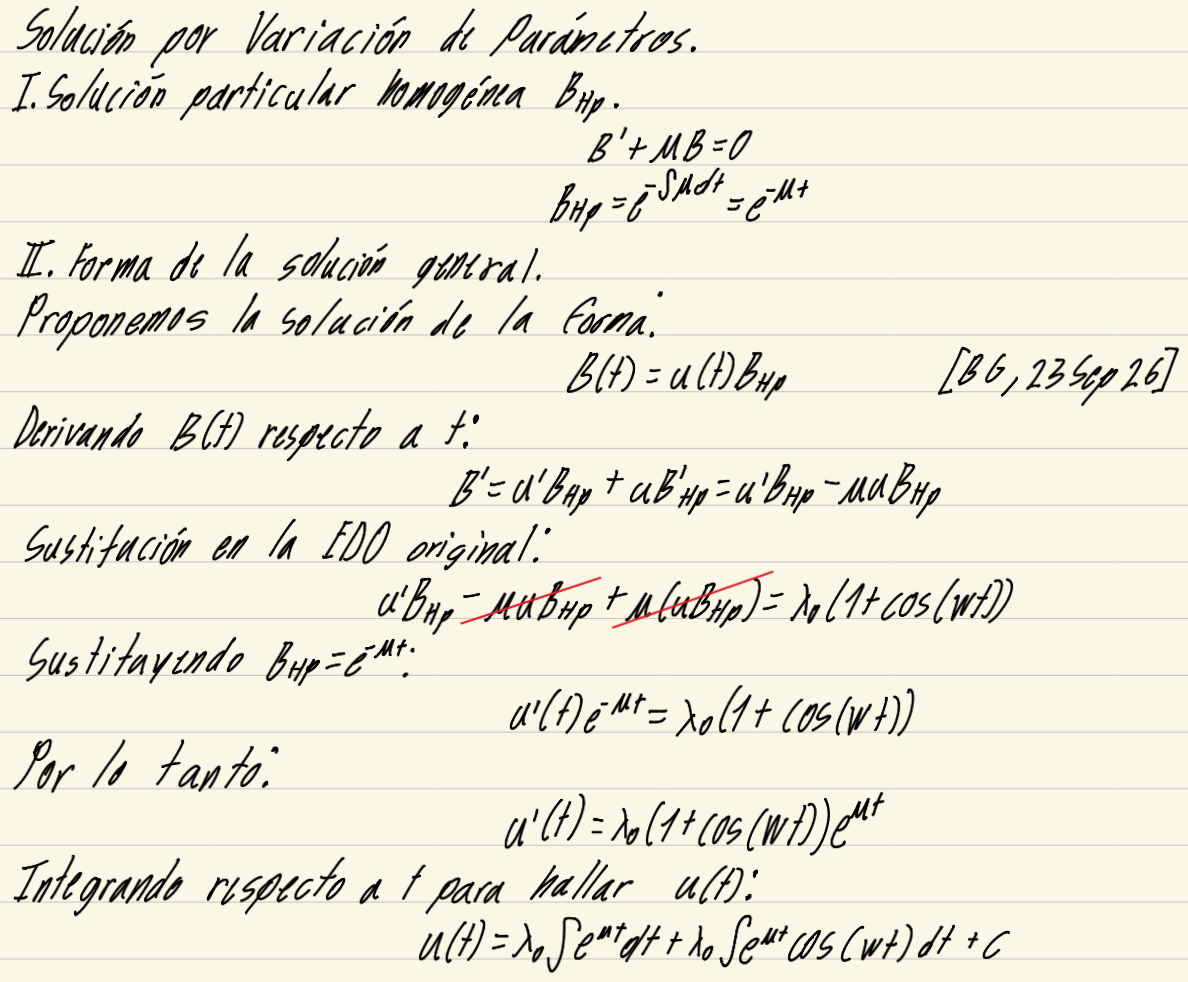
\includegraphics[width=0.8\linewidth]{imagenes/tarea/03_ejercicio/02_image.png}
    \end{figure}

    \begin{figure}[H]
        \centering
        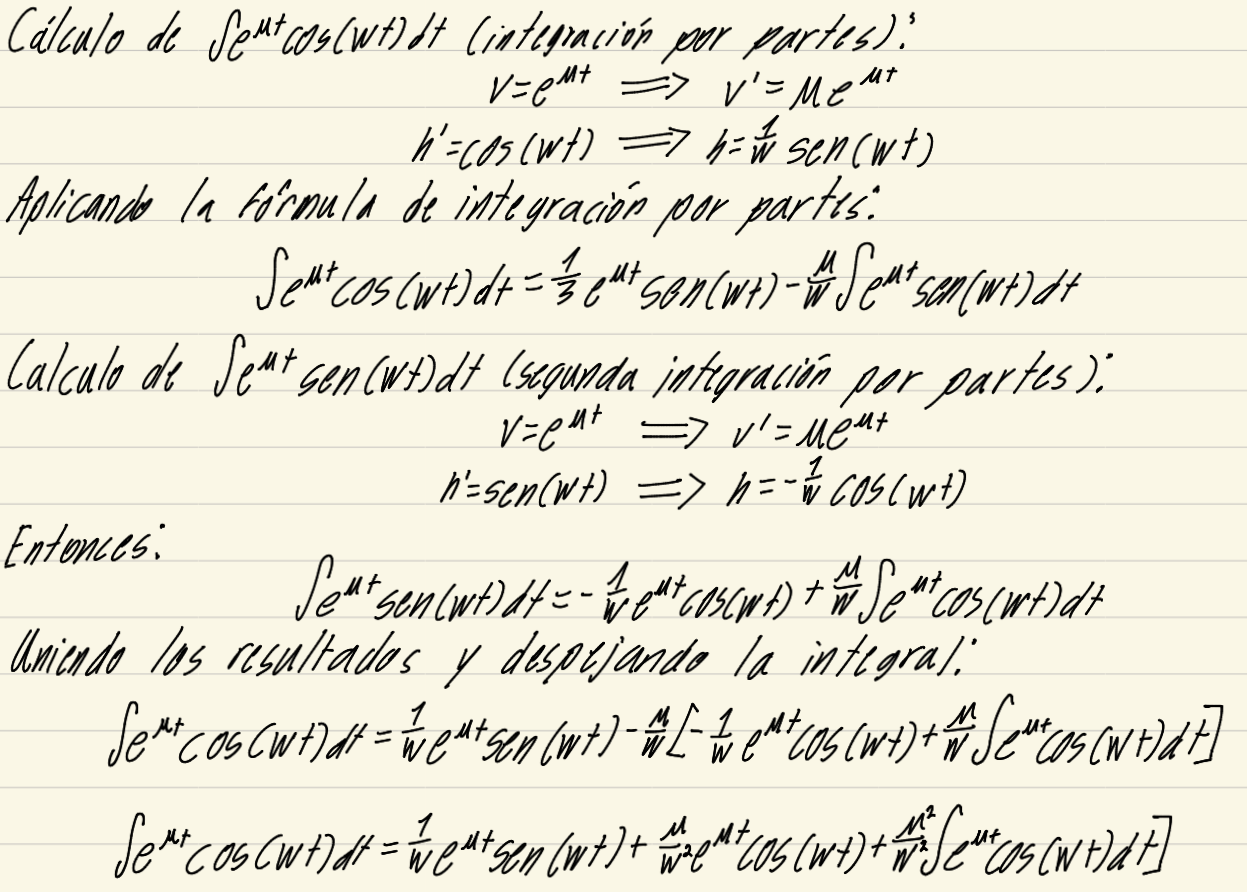
\includegraphics[width=0.8\linewidth]{imagenes/tarea/03_ejercicio/03_image.png}
    \end{figure}

    \begin{figure}[H]
        \centering
        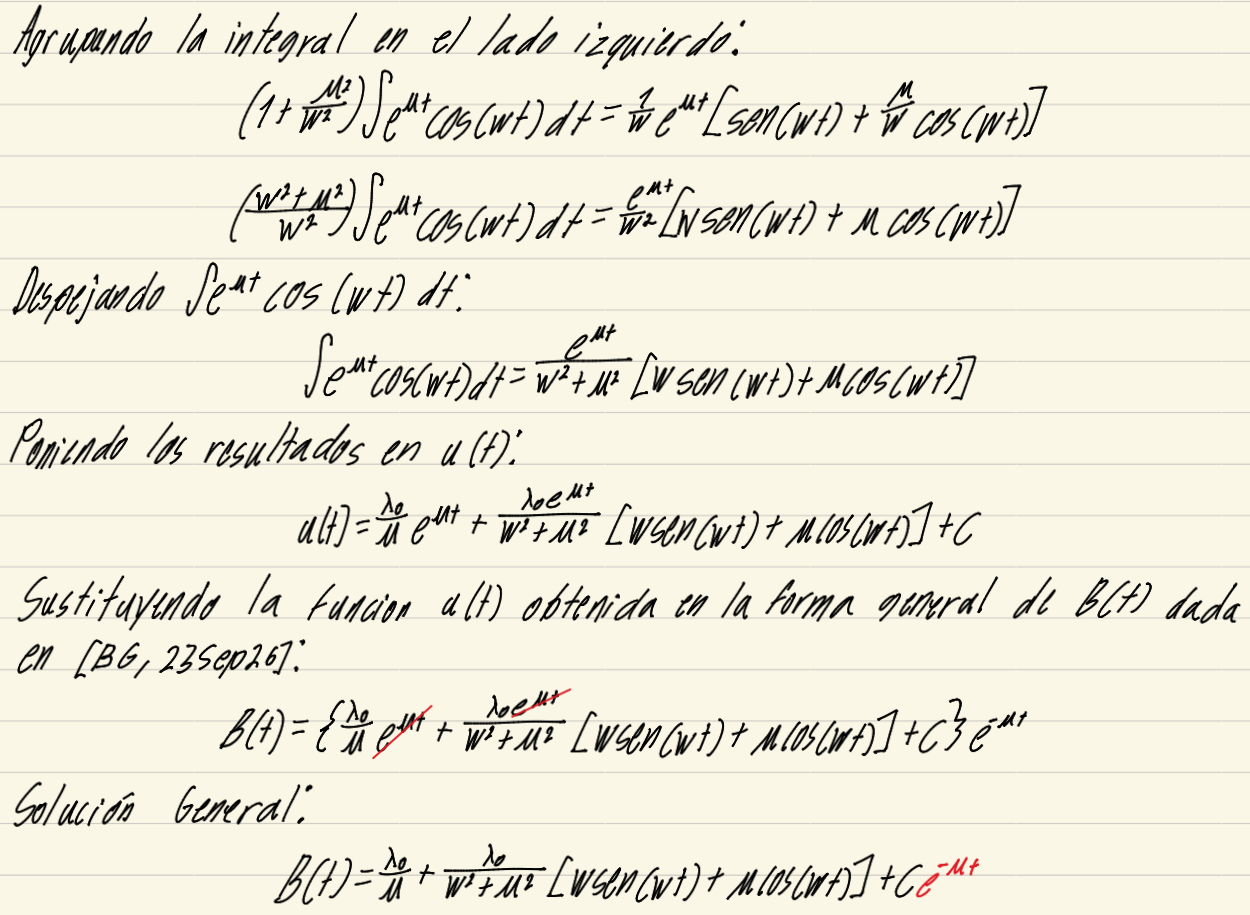
\includegraphics[width=0.8\linewidth]{imagenes/tarea/03_ejercicio/04_image.png}
    \end{figure}

    \begin{figure}[H]
        \centering
        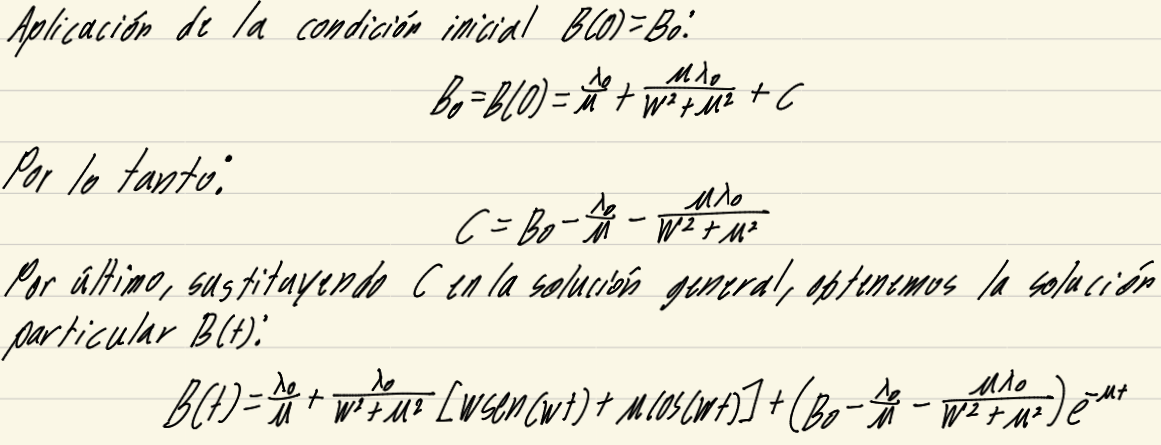
\includegraphics[width=0.8\linewidth]{imagenes/tarea/03_ejercicio/05_image.png}
    \end{figure}

    \item \textbf{Pérdida de paquetes con recuperación variable en una red.} \\
    Toma la EDO y valores de este problema dados en la clase del 28 de Septiembre (Video 4), pero ahora resuelve por el Método de Variación de Parámetros.
    \subsection*{Solución}
    \begin{figure}[H]
        \centering
        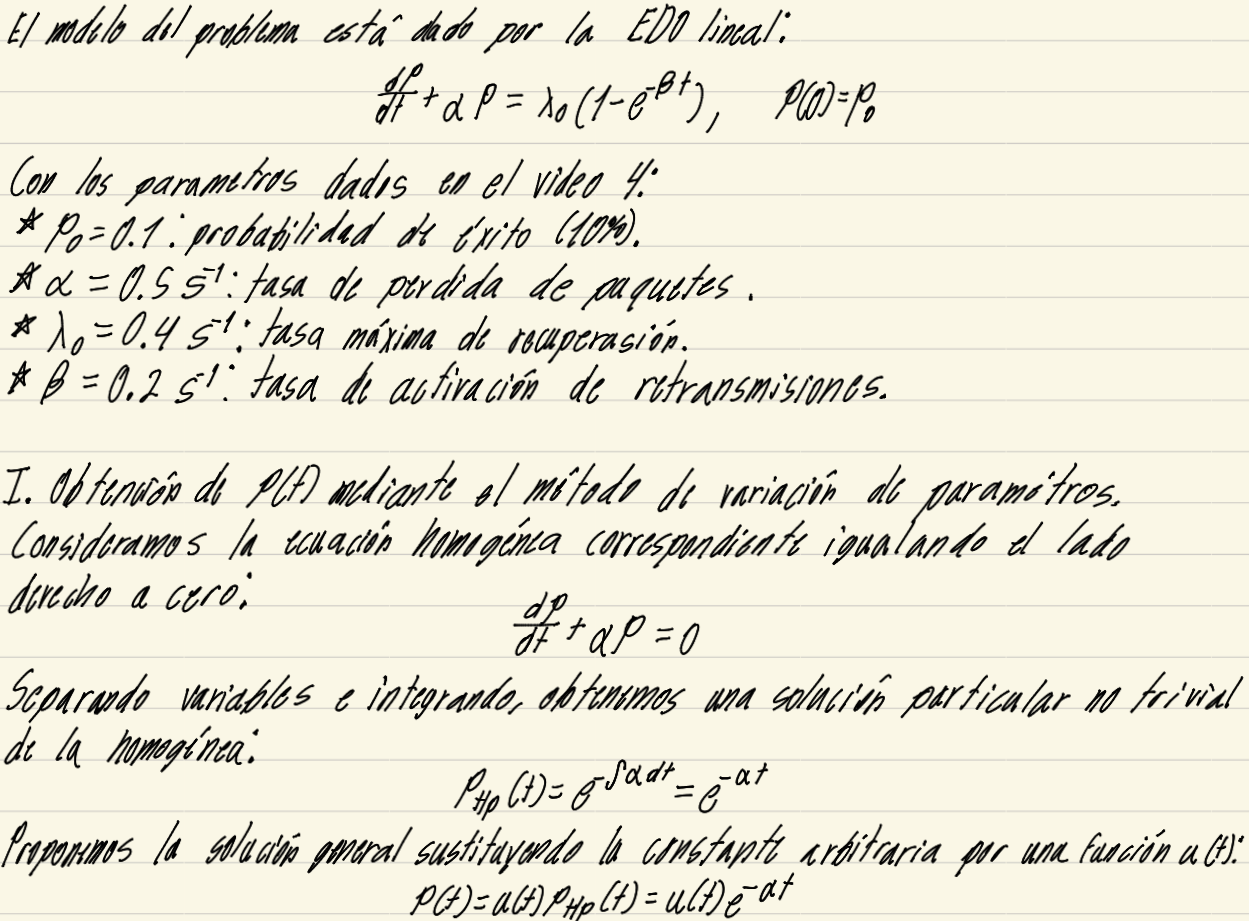
\includegraphics[width=0.9\linewidth]{imagenes/tarea/03_ejercicio/06_image.png}
    \end{figure}

    \begin{figure}[H]
        \centering
        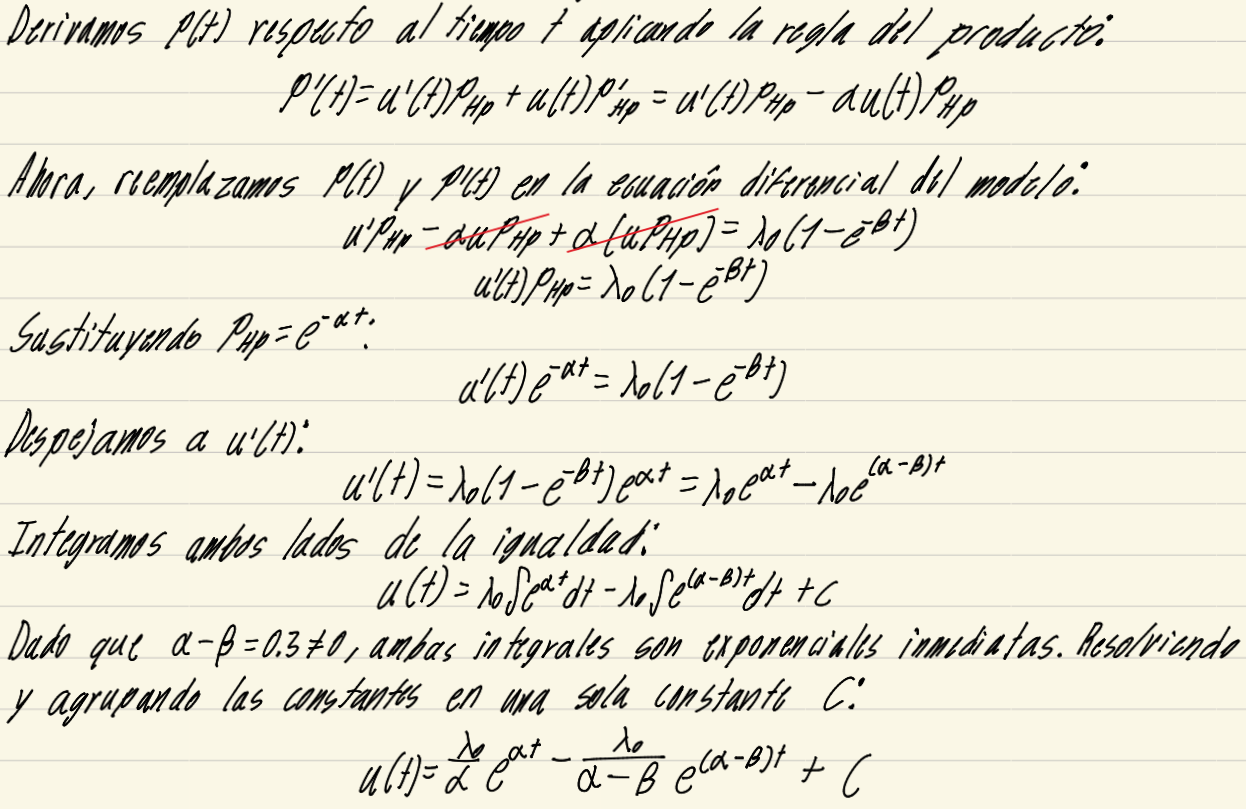
\includegraphics[width=0.9\linewidth]{imagenes/tarea/03_ejercicio/07_image.png}
    \end{figure}

    \begin{figure}[H]
        \centering
        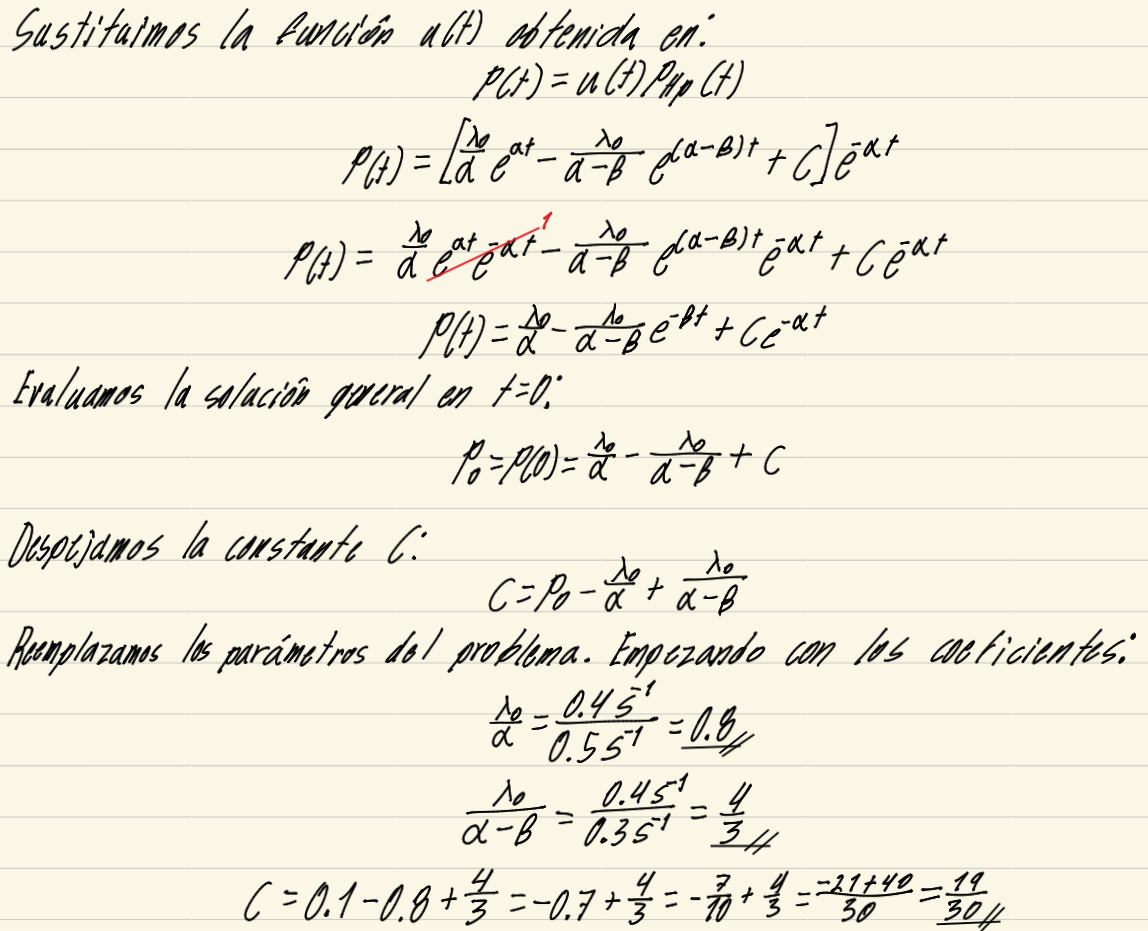
\includegraphics[width=0.9\linewidth]{imagenes/tarea/03_ejercicio/08_image.png}
    \end{figure}

    \begin{figure}[H]
        \centering
        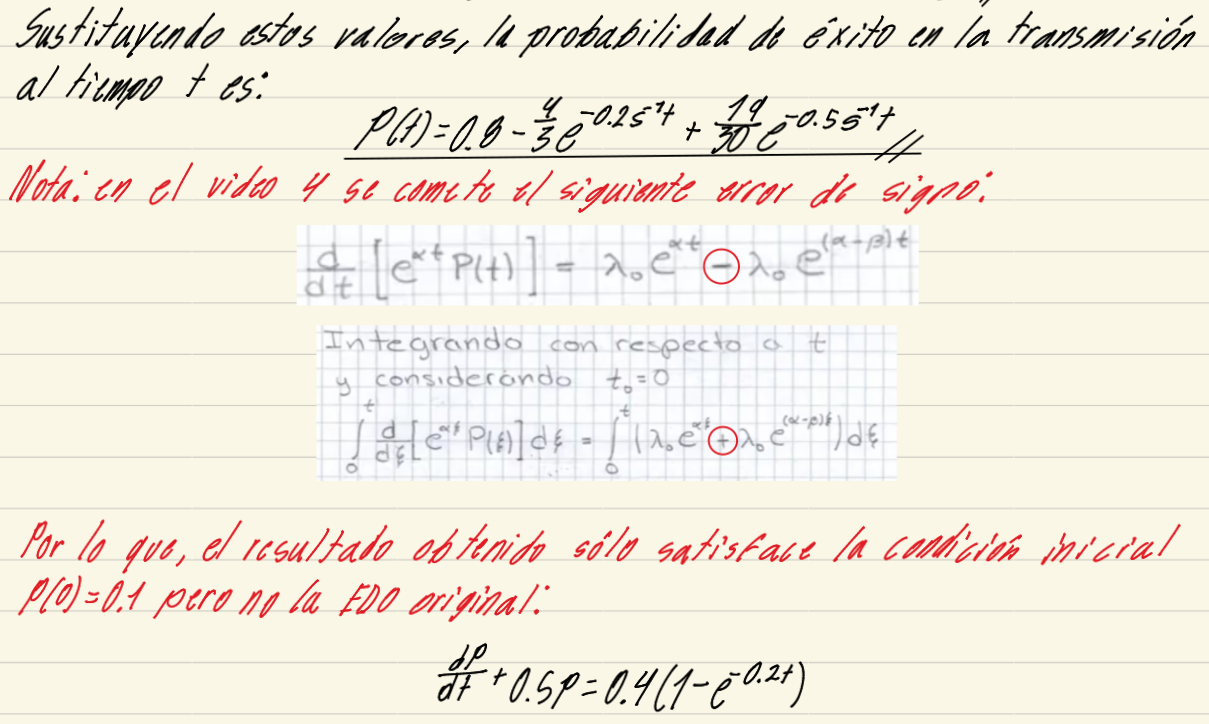
\includegraphics[width=0.9\linewidth]{imagenes/tarea/03_ejercicio/09_image.png}
    \end{figure}

    \begin{figure}[H]
        \centering
        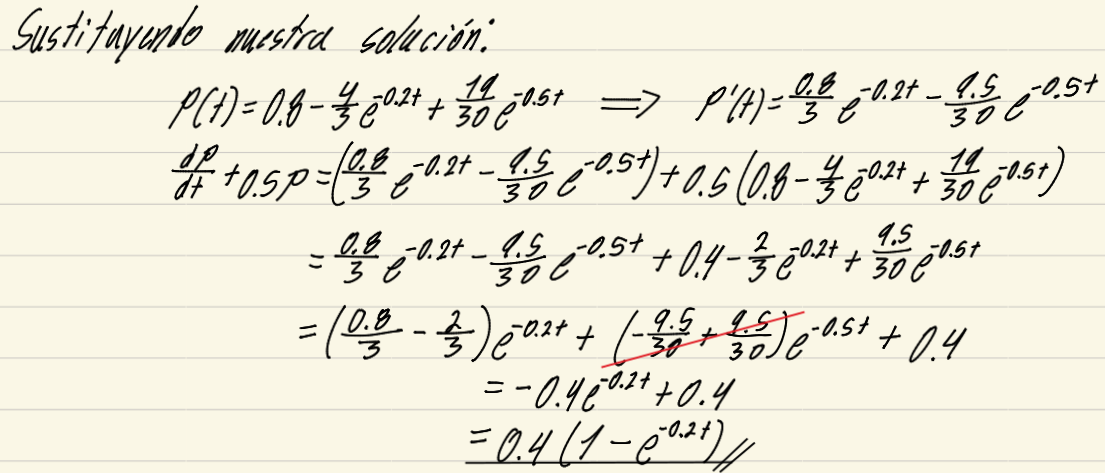
\includegraphics[width=0.9\linewidth]{imagenes/tarea/03_ejercicio/10_image.png}
    \end{figure}

    \begin{figure}[H]
        \centering
        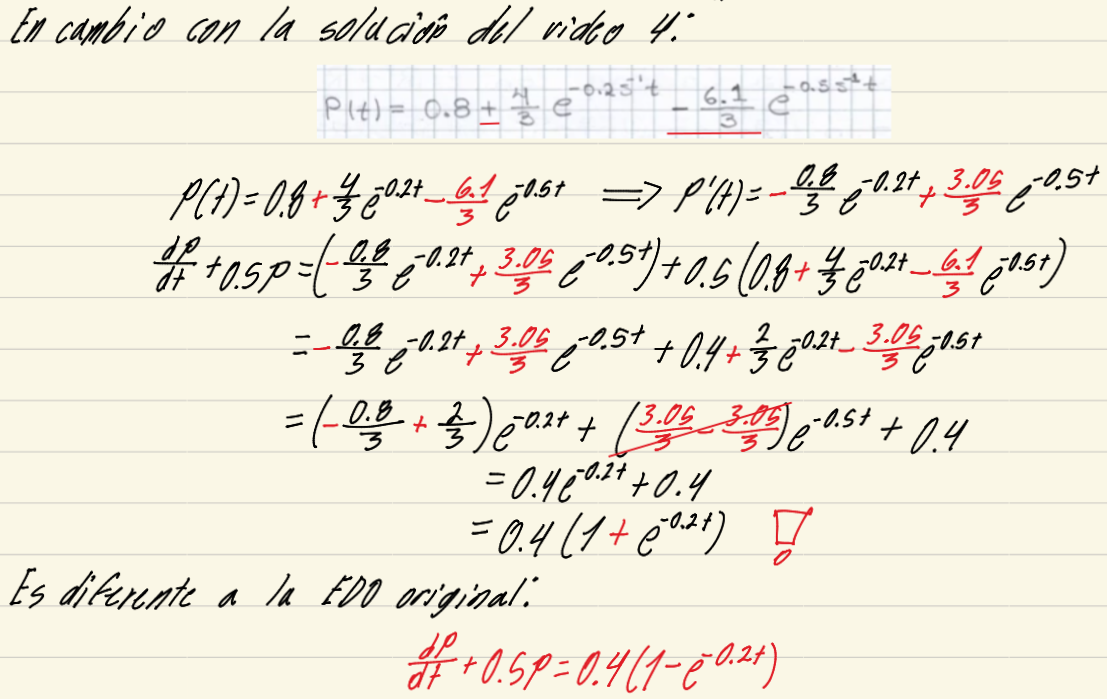
\includegraphics[width=0.9\linewidth]{imagenes/tarea/03_ejercicio/11_image.png}
    \end{figure}

    \item \textbf{Temperatura en un Procesador con Potencia Variable.}

    En un procesador moderno (CPU o GPU), la temperatura $T(t)$ no es constante: depende de la carga de trabajo y de la capacidad del sistema de enfriamiento para disipar el calor generado. Cuando el procesador ejecuta tareas, consume energía eléctrica que se transforma casi por completo en calor; sin embargo, la carga de trabajo no suele ser constante: en muchos escenarios reales (servidores web, videojuegos, aplicaciones de inteligencia artificial, centros de datos), la demanda de cómputo fluctúa de forma periódica o cuasi-periódica, con ciclos de alta y baja actividad.

    Esta variación en la carga se traduce en una potencia disipada variable $P(t)$, que podemos modelar como una señal sinusoidal alrededor de un valor base $P_{0}$:
    \[ P(t) = P_{0}(1 + \operatorname{sen}(\omega t)) \]
    donde:
    \begin{itemize}[leftmargin=*]
        \item $P_{0}$ es la potencia media o base dada en watts ($\text{W}$),
        \item $\omega$ es la frecuencia angular de la variación ($\text{rad/s}$), que refleja qué tan rápido cambia la carga.
    \end{itemize}

    Por otro lado, el procesador se enfría hacia la temperatura ambiente $T_{\text{amb}}$ mediante mecanismos de disipación (ventiladores, disipadores, líquido refrigerante). La ley de enfriamiento de Newton establece que la tasa de pérdida de calor es proporcional a la diferencia entre la temperatura actual y la ambiente:
    \[ \text{Enfriamiento} \propto -k(T - T_{\text{amb}}) \]
    donde $k$ es la constante de enfriamiento ($1/\text{s}$), que depende del diseño térmico del sistema.

    Combinando ambos efectos (calentamiento por potencia variable y enfriamiento por ley de Newton), se obtiene la ecuación diferencial que describe la evolución de la temperatura:
    \[ \frac{dT}{dt} = -k(T - T_{\text{amb}}) + \frac{P(t)}{C} \]

    Sustituyendo $P(t) = P_{0}(1 + \operatorname{sen}(\omega t))$ y reordenando, obtenemos la EDO que modela el cambio de Temperatura en un Procesador con Potencia Variable:
    \begin{equation*}
        \frac{dT}{dt} + kT = kT_{\text{amb}} + \frac{P_{0}}{C}(1 + \operatorname{sen}(\omega t)) \tag{TP.PV}
    \end{equation*}
    donde $C$ es la capacidad calorífica del procesador ($\text{J/K}$) que indica cuánta energía se necesita para elevar su temperatura en $1\text{ K}$ ($\text{J} \equiv \text{Joules}$; $\text{K} \equiv \text{Kelvin}$).

    Tomando los siguientes valores, resuelve la EDO \texttt{TP.PV} por el Método de Factor Integrante (Segundo Video):

    \vspace{0.3cm}
    \begin{center}
    \resizebox{\linewidth}{!}{
    \begin{tabular}{c c c p{7.5cm}}
    \toprule
    \textbf{Parámetro} & \textbf{Valor} & \textbf{Unidades} & \textbf{Interpretación} \\
    \midrule
    $T_{\text{amb}}$ & $25$ & $^{\circ}\text{C}$ & Temperatura ambiente típica de un centro de datos \\
    \addlinespace
    $P_{0}$ & $65$ & $\text{W}$ & Potencia base de un procesador de escritorio \\
    \addlinespace
    $C$ & $100$ & $\text{J/K}$ & Capacidad calorífica típica de un disipador \\
    \addlinespace
    $k$ & $0.1$ & $\text{s}^{-1}$ & Constante de enfriamiento con ventilador activo \\
    \addlinespace
    $\omega$ & $0.5$ & $\text{rad/s}$ & Variación de carga cada $12.6\text{ s}$ \\
    \addlinespace
    $T(0)$ & $40$ & $^{\circ}\text{C}$ & Temperatura inicial del procesador \\
    \bottomrule
    \end{tabular}
    }
    \end{center}
    \vspace{0.3cm}

    siguiendo los siguientes pasos:
    \begin{enumerate}[label=(\alph*), leftmargin=*]
        \item Identifique $a(t)$ y $f(t)$.
        \subsection*{Solución}
        \begin{figure}[H]
            \centering
            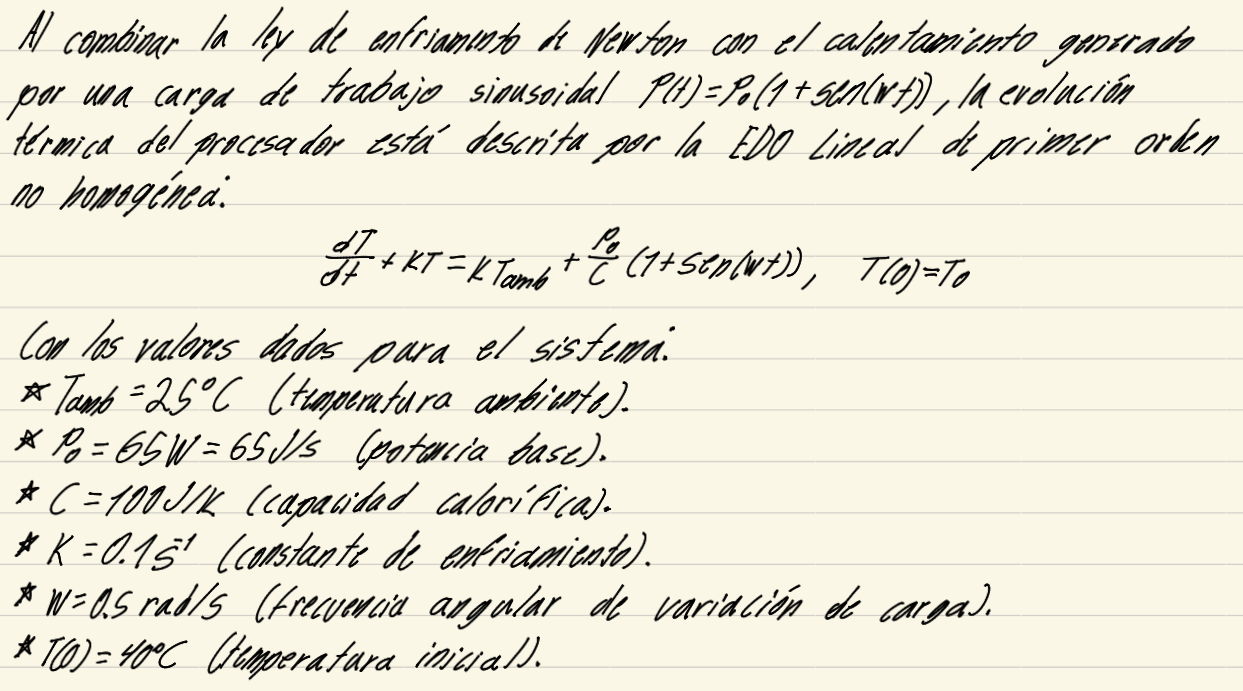
\includegraphics[width=0.9\linewidth]{imagenes/tarea/03_ejercicio/12_image.png}
        \end{figure}

        \begin{figure}[H]
            \centering
            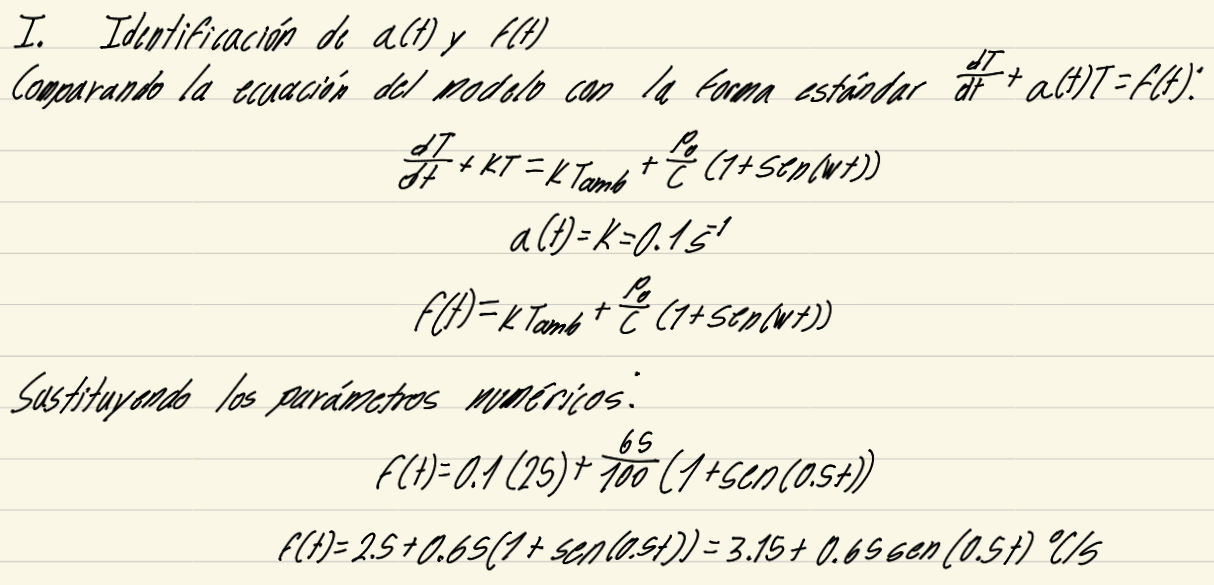
\includegraphics[width=0.9\linewidth]{imagenes/tarea/03_ejercicio/13_image.png}
        \end{figure}

        \item Encuentra $T(t)$ por el Método de Factor Integrante.
        \subsection*{Solución}
        \begin{figure}[H]
            \centering
            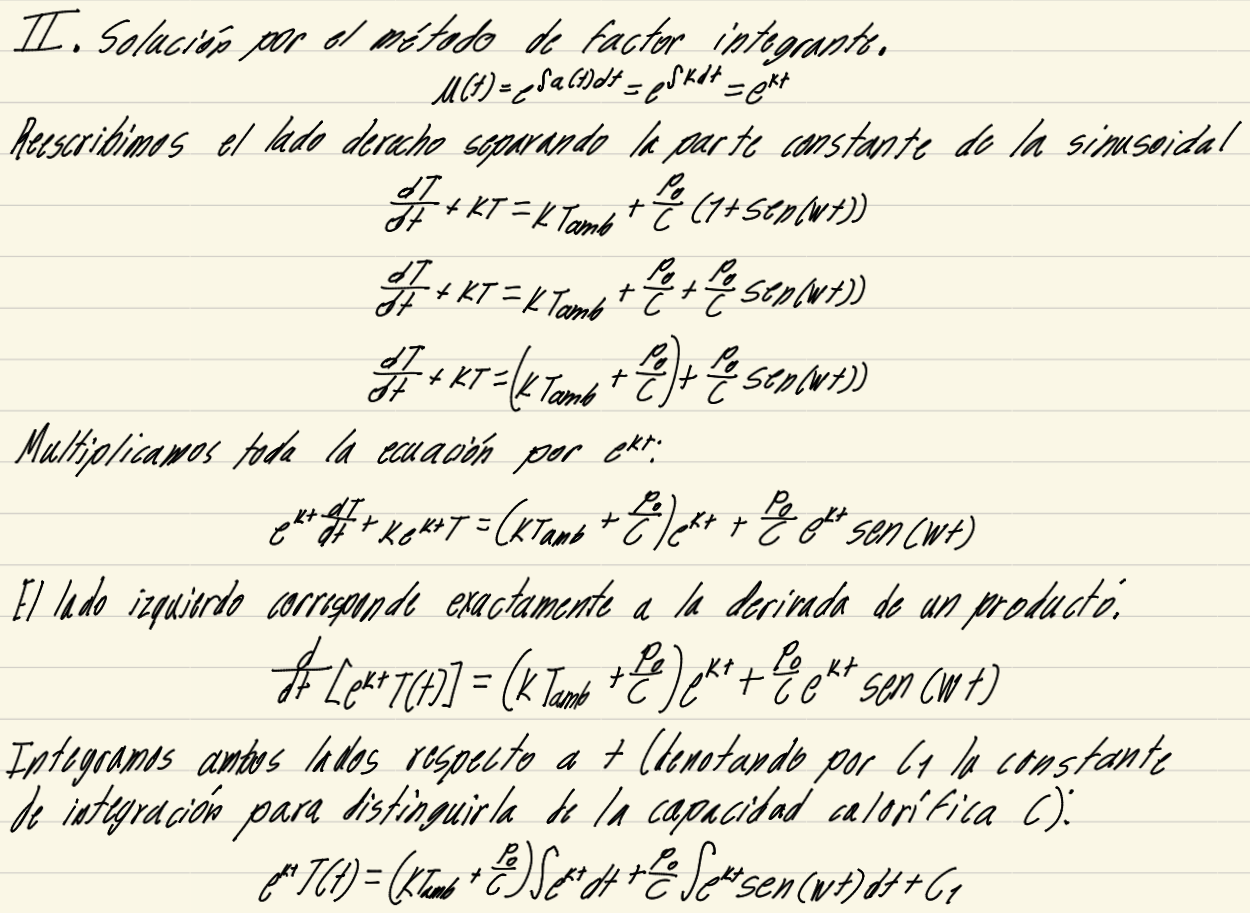
\includegraphics[width=0.9\linewidth]{imagenes/tarea/03_ejercicio/14_image.png}
        \end{figure}

        \begin{figure}[H]
            \centering
            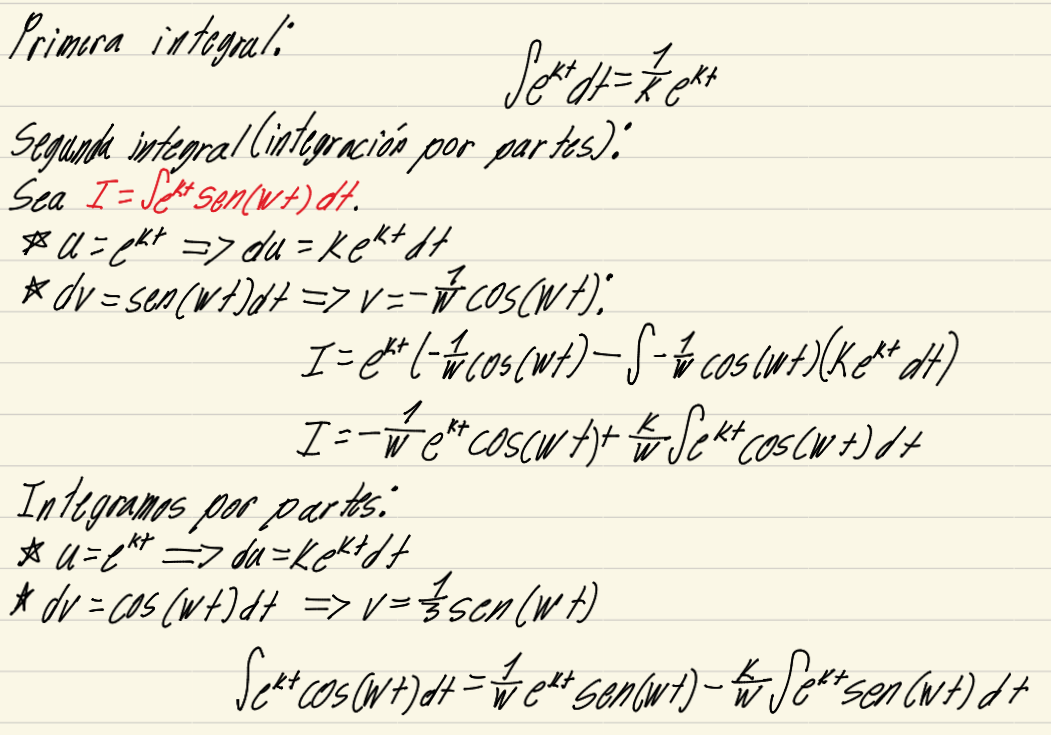
\includegraphics[width=0.9\linewidth]{imagenes/tarea/03_ejercicio/15_image.png}
        \end{figure}

        \begin{figure}[H]
            \centering
            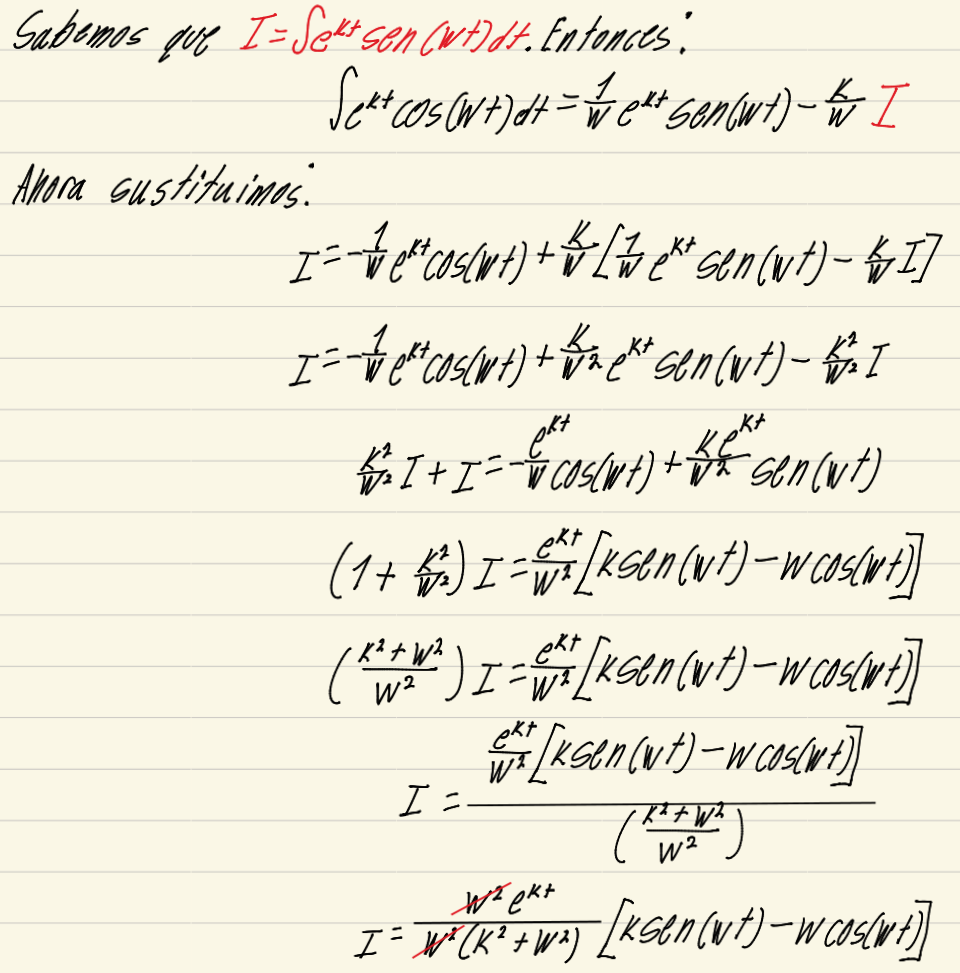
\includegraphics[width=0.9\linewidth]{imagenes/tarea/03_ejercicio/16_image.png}
        \end{figure}

        \begin{figure}[H]
            \centering
            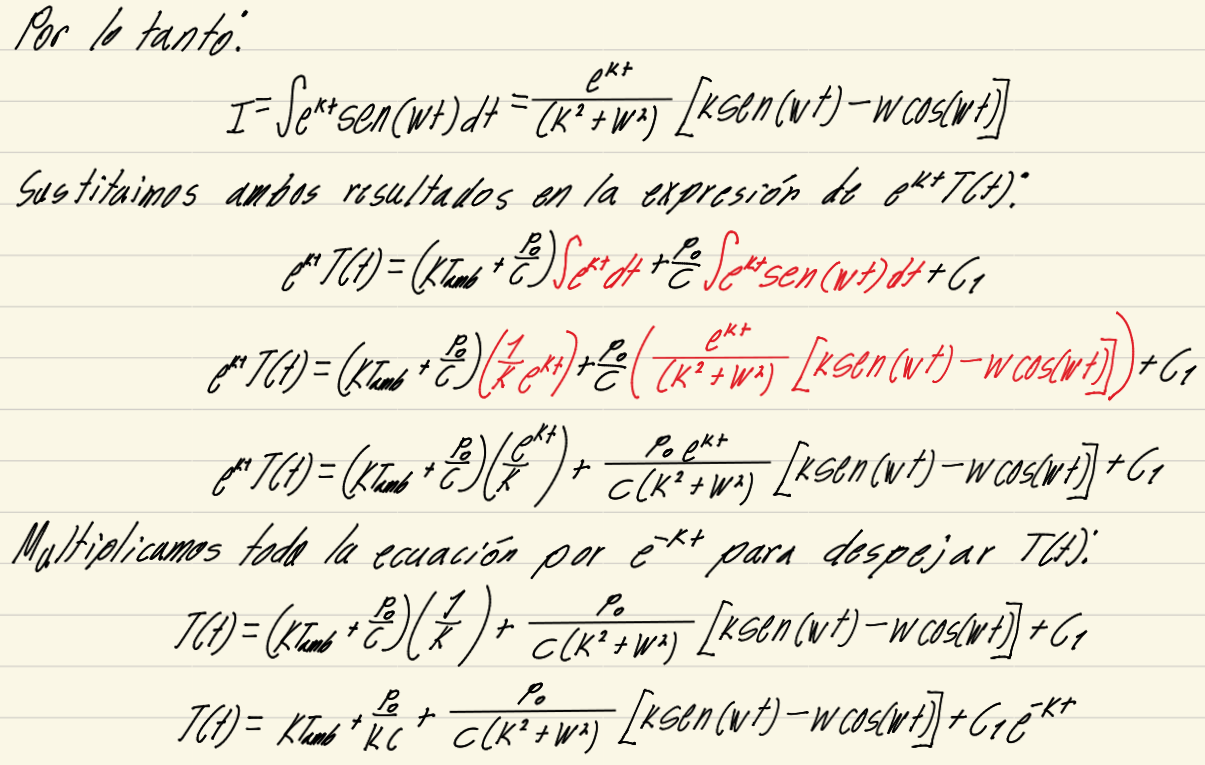
\includegraphics[width=0.9\linewidth]{imagenes/tarea/03_ejercicio/17_image.png}
        \end{figure}

        \begin{figure}[H]
            \centering
            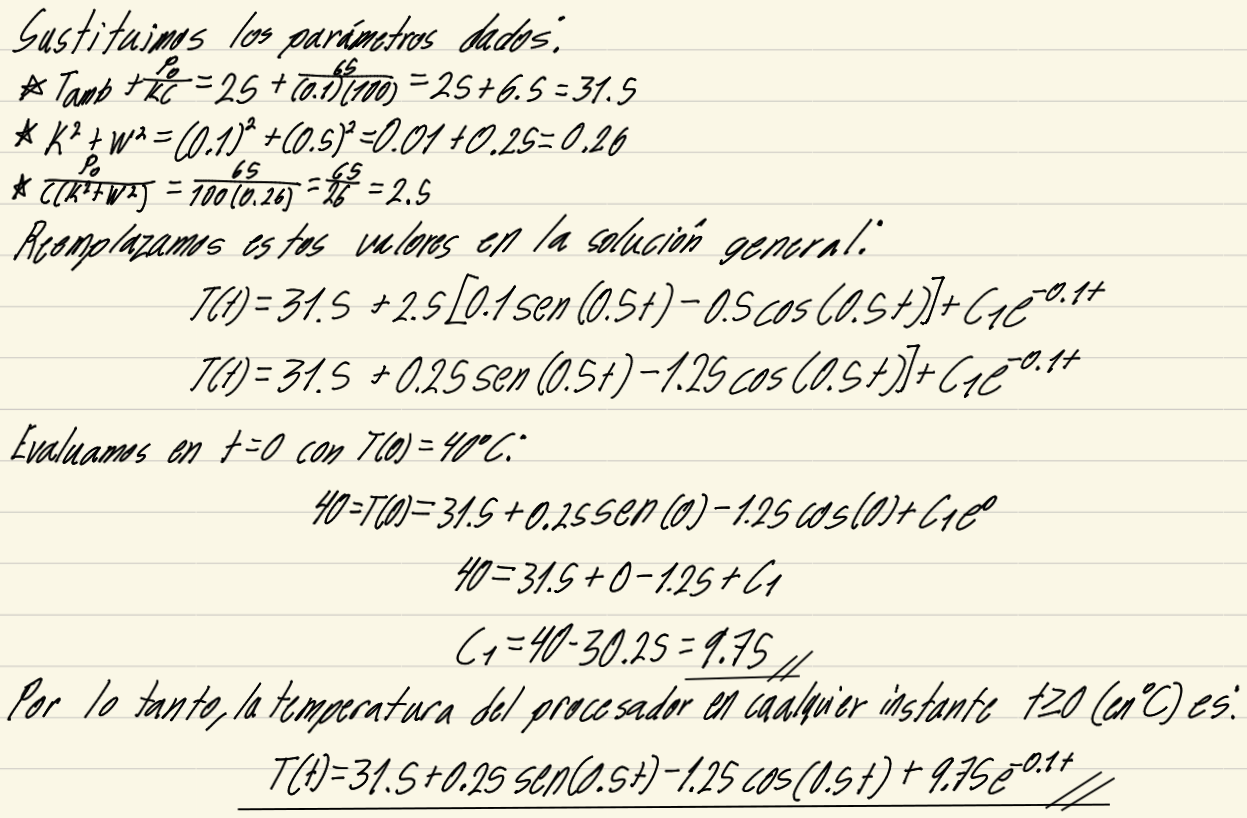
\includegraphics[width=0.9\linewidth]{imagenes/tarea/03_ejercicio/18_image.png}
        \end{figure}

        \item Determine la temperatura de equilibrio.
        \subsection*{Solución}

        \begin{figure}[H]
            \centering
            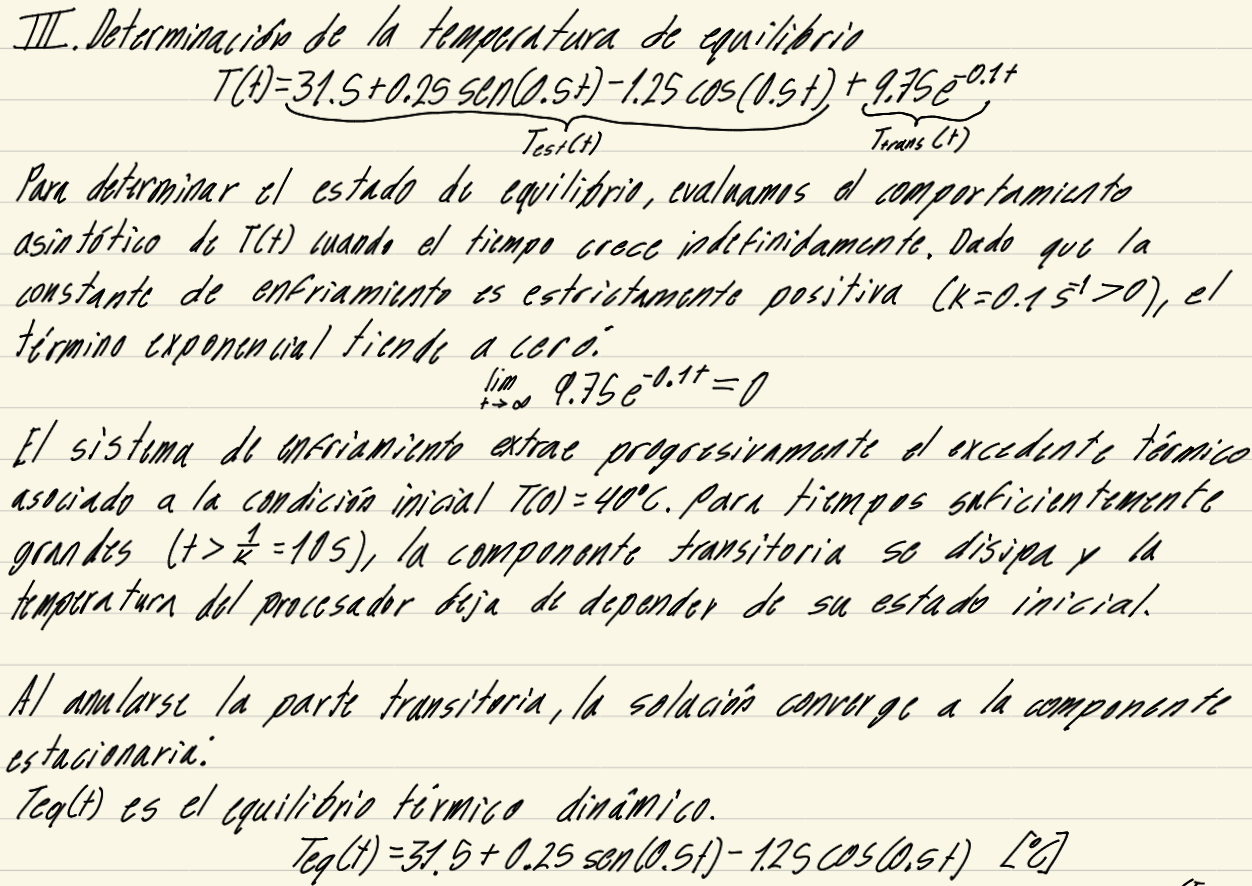
\includegraphics[width=0.9\linewidth]{imagenes/tarea/03_ejercicio/19_image.png}
        \end{figure}

        \begin{figure}[H]
            \centering
            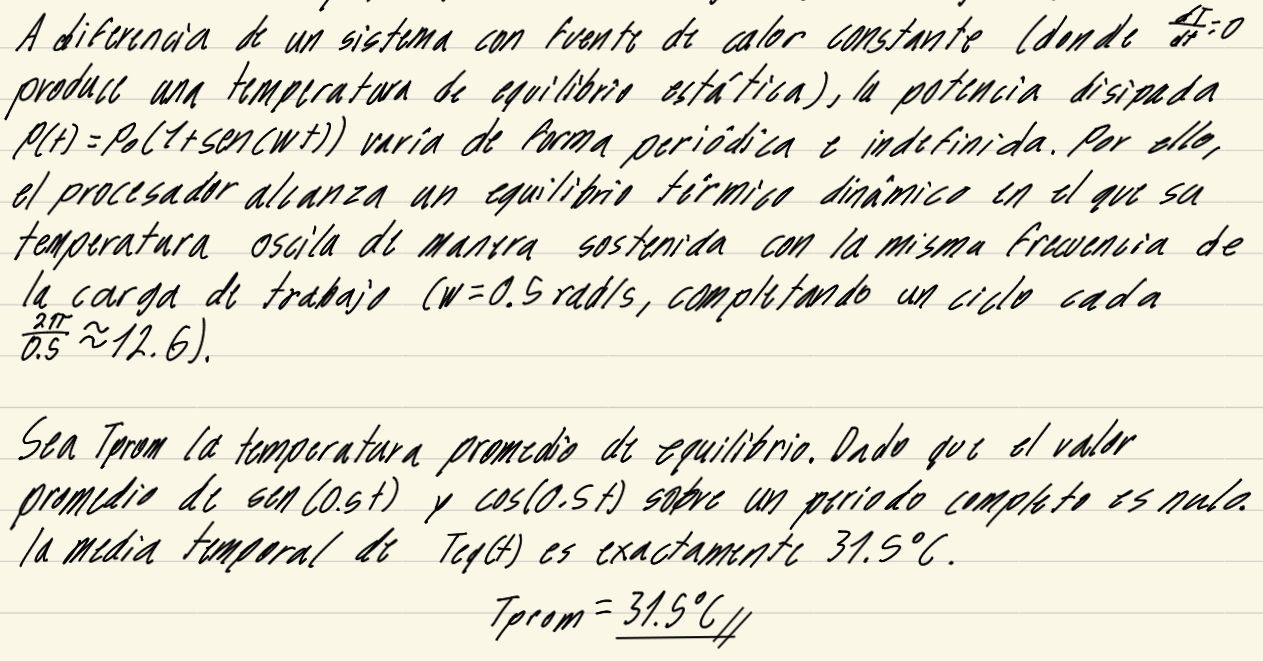
\includegraphics[width=0.9\linewidth]{imagenes/tarea/03_ejercicio/20_image.png}
        \end{figure}
    \end{enumerate}
\end{enumerate}